\documentclass[10pt,a4paper,oneside]{article}
\usepackage[utf8]{inputenc} 
\usepackage[russian]{babel}
\usepackage{amsmath,amssymb}
\usepackage{amsthm}
\usepackage{amsfonts}
\usepackage{tipa}
\usepackage{hyperref}
\usepackage{tikz}
\usepackage{stmaryrd}
\usepackage{mathtools}
\usepackage{graphicx}
\usepackage{indentfirst}
\usepackage{cmll}
\usepackage{comment}
\usepackage{fancyhdr}
\usepackage{proof}
\usepackage[tocflat]{tocbasic}
\usepackage{titlesec}
\usepackage{minted}
\newcommand{\sectionbreak}{\clearpage}
\usepackage{float}
\usepackage{enumerate}
\binoppenalty=10000
\relpenalty=10000
\usepackage{multicol}
\usepackage{enumitem}
\usepackage{ulem}
\usepackage{cancel}
\usepackage{pdfpages}
\usepackage[left=2cm,right=2cm,
    top=2cm,bottom=2cm,bindingoffset=0cm]{geometry}
\usepackage{xcolor}
\definecolor{linkcolor}{HTML}{2832C2} % цвет ссылок
\definecolor{urlcolor}{HTML}{2832C2} % цвет гиперссылок
\hypersetup{pdfstartview=FitH,  linkcolor=linkcolor,urlcolor=urlcolor, colorlinks=true}
\setlength{\parindent}{5ex}

\titleformat{\section}[block]{\Large\bfseries\filcenter}{}{1em}{}

\makeatletter
\newcommand{\dotminus}{\mathbin{\text{\@dotminus}}}

\makeatletter
\renewcommand\l@section{\@dottedtocline{1}{1.5em}{3.0em}}
\renewcommand\l@subsection{\@dottedtocline{1}{1.5em}{3.0em}}
\makeatother

\newcommand{\fash}[1]{%
    \begin{tikzpicture}[#1]
        \draw (-1,1)  -- (-1,0) -- (1,0) -- (1,-1);
        \draw (-1,-1) -- (0,-1) -- (0,1) -- (1,1);
    \end{tikzpicture}%
}

\DeclareMathOperator*{\argmax}{arg\,max}
\DeclareMathOperator*{\argmin}{arg\,min}

\newtheorem{definition}{Определение}

\title{Лабораторная работа №2.  Ручное построение
нисходящих синтаксических анализаторов }
\author{Юльцова Наталья М33351}

\begin{document}

  \pagenumbering{gobble}
  \maketitle
  \pagenumbering{arabic}
  
  \section{1. Разработка грамматики}
  \noindent 
  Вариант 7: Описание переменных в Си\\\\
  На вход подаются строки типа : $type_1$ $var_1$, ... $var_k$; $type_2$  ... \\
  Бывают простые переменные и указатели(т.е звездочка* переменная). По условию, используем один терминал для переменных и типов - обозначим за v.\\\\
  
  Построим грамматику:\\
  
  $$S \rightarrow vFL \ ;S \ | \ \varepsilon$$
  $$L \rightarrow \ ,FL\ | \ \varepsilon$$
  $$F \rightarrow  *F \ | \ v$$ 
  
  \begin{center}
      \begin{tabular}{ | l | l | }
      \hline
      Нетерминал & Описание \\ \hline
      S & Описание переменных \\ \hline
      L & Описание переменных через запятую \\ \hline
      F & Переменная или указатель \\ \hline
      \end{tabular}
  \end{center}
  
   В грамматике нет левой рекурсии или правого ветвления, поэтому она остается без изменений.
  
  \section{2. Построение лексического анализатора}
  \noindent
  В нашей грамматике есть следующие терминалы:
  \begin{itemize}
      \item * -- указатель
      \item ; -- разделяет типы
      \item , -- разделяет переменные
      \item v -- имя переменной или типа
      \item \$ -- конец
  \end{itemize}
  
  \noindent
  Построим лексический анализатор. Заведем класс Token для хранения терминалов, в том числе конец строки.\\
  \begin{verbatim}
    public enum Token {
        STAR, SEMICOLON, COMMA, NAME, END
    }
  \end{verbatim}
  
   \begin{center}
      \begin{tabular}{ | l | l | }
      \hline
      Терминал & TOKEN \\ \hline
      * & STAR \\ \hline
      ; & SEMICOLON \\ \hline
      , & COMMA \\ \hline
      v & NAME \\ \hline
      \$ & END \\ \hline
      \end{tabular}
  \end{center}
  
  \noindent
  Лексический анализатор:
  \begin{verbatim}
        import java.io.IOException;
        import java.io.InputStream;
        import java.text.ParseException;
        
        public class LexicalAnalyser {
            private final InputStream is;
            private int curChar;
            private int curPos;
            private Token curToken;
        
            public LexicalAnalyser(InputStream is) throws ParseException {
                this.is = is;
                curPos = 0;
                nextChar();
            }
        
            private boolean isBlank(int c) {
                return Character.isWhitespace(c);
            }
        
            private void nextChar() throws ParseException {
                curPos++;
                try {
                    curChar = is.read();
                } catch (IOException e) {
                    throw new ParseException(e.getMessage(), curPos);
                }
            }
        
            public String nextToken() throws ParseException {
                while (isBlank(curChar)) {
                    nextChar();
                }
        
                switch (curChar) {
                    case '*':
                        nextChar();
                        curToken = Token.STAR;
                        return "*";
                    case ';':
                        nextChar();
                        curToken = Token.SEMICOLON;
                        return ";";
                    case ',':
                        nextChar();
                        curToken = Token.COMMA;
                        return ",";
                    case '$':
                        curToken = Token.END;
                        return "$";
                    default:
                        if (!Character.isAlphabetic(curChar)) {
                            throw new ParseException("Invalid token at pos " + curPos, curPos());
                        }
                        StringBuilder token = new StringBuilder();
                        while (Character.isAlphabetic(curChar) || Character.isDigit(curChar) || curChar == '_') {
                            token.append(Character.toChars(curChar));
                            nextChar();
                        }
                        curToken = Token.NAME;
                        return token.toString();
                }
            }
        
            public Token curToken() {
                return curToken;
            }
        
            public int curPos() {
                return curPos;
            }
        }
  \end{verbatim}
  
  \section{3. Построение синтаксического анализатора}
  \noindent
  Построим множества FIRST и FOLLOW для нетерминалов нашей грамматики.
  
  \begin{center}
      \begin{tabular}{|l|l|l|}
      \hline
        Нетерминал & FIRST            & FOLLOW \\ \hline
        S          & v \varepsilon    & \$     \\ \hline
        L          & , \varepsilon    &  ;     \\ \hline
        F          & v *              &  , ;  \\ \hline
      \end{tabular}
  \end{center}
  
  Заведем структуру для хранения дерева:
  \begin{verbatim}
    import java.util.ArrayList;
    import java.util.Arrays;
    import java.util.List;
    
    public class Tree {
        String node;
        List<Tree> children;
    
        public Tree(String node, Tree... children) {
            this.node = node;
            this.children = Arrays.asList(children);
        }
    
        public Tree(String node) {
            this.node = node;
            children = new ArrayList<>();
        }
    
        @Override
        public String toString() {
            StringBuilder ans = new StringBuilder();
            for (Tree t : children) {
                ans.append(node).append("->").append(t.node).append(";").append("\n").append(t.toString());
            }
            return ans.toString();
        }
    }
  \end{verbatim}
  
  Синтаксический анализатор с использованием рекурсивного спуска:
  \begin{verbatim}
        import java.io.InputStream;
        import java.text.ParseException;
        
        public class Parser {
            private LexicalAnalyser lex;
            private String token;
        
            private Tree S() throws ParseException {
                if (lex.curToken() == Token.NAME) {
                    String name = token;
                    token = lex.nextToken();
                    Tree f = F();
                    token = lex.nextToken();
                    Tree l = L();
                    if (lex.curToken() != Token.SEMICOLON) {
                        throw new ParseException("`;` expected at pos " + lex.curPos(), lex.curPos());
                    }
                    token = lex.nextToken();
                    Tree s = S();
                    if (lex.curToken() != Token.END) {
                        throw new ParseException("Eof expected at pos " + lex.curPos(), lex.curPos());
                    }
                    return new Tree("S", new Tree(name), f, l, new Tree("SEMICOLON"), s);
                } else if (lex.curToken() == Token.END) {
                    return new Tree("S", new Tree("eps"));
                } else
                    throw new ParseException("Expression expected at pos " + lex.curPos(), lex.curPos());
            }
        
            private Tree L() throws ParseException {
                if (lex.curToken() == Token.SEMICOLON) {
                    return new Tree("L", new Tree("eps"));
                } else if (lex.curToken() == Token.COMMA) {
                    token = lex.nextToken();
                    Tree f = F();
                    token = lex.nextToken();
                    Tree l = L();
                    return new Tree("L", new Tree("COMMA"), f, l);
                }
                throw new ParseException("Expected ; or , at pos " + lex.curPos(), lex.curPos());
            }
        
            private Tree F() throws ParseException {
                if (lex.curToken() == Token.STAR) {
                    token = lex.nextToken();
                    Tree f = F();
                    return new Tree("F", new Tree("STAR"), f);
                } else if (lex.curToken() == Token.NAME) {
                    String name = token;
                    return new Tree("F", new Tree(name));
                }
                throw new ParseException("Varname is incorrect. Unexpected token at pos " + lex.curPos(), lex.curPos());
            }
        
        
            public Tree parse(InputStream is) throws ParseException {
                lex = new LexicalAnalyser(is);
                token = lex.nextToken();
                return S();
            }
        }
        
    Запуск:
    
        import java.text.ParseException
        public class Main {
            public static void main(String[] args) throws ParseException {
                final Parser parser = new Parser();
                System.out.println(parser.parse(System.in).toString());
            }
        }

  \end{verbatim}
  \section{4. Визуализация дерева разбора}
  \noindent
  Для изучения результата будем использовать систему GraphViz
(https://graphviz.org/) и рассмотримм полученное в ходе тестирования дерево.\\\\

Пример на различные правила: \\
int64\_t a; \\
boolean true, FaL\_s3e; \\
char *x, ***y;\$ \\

    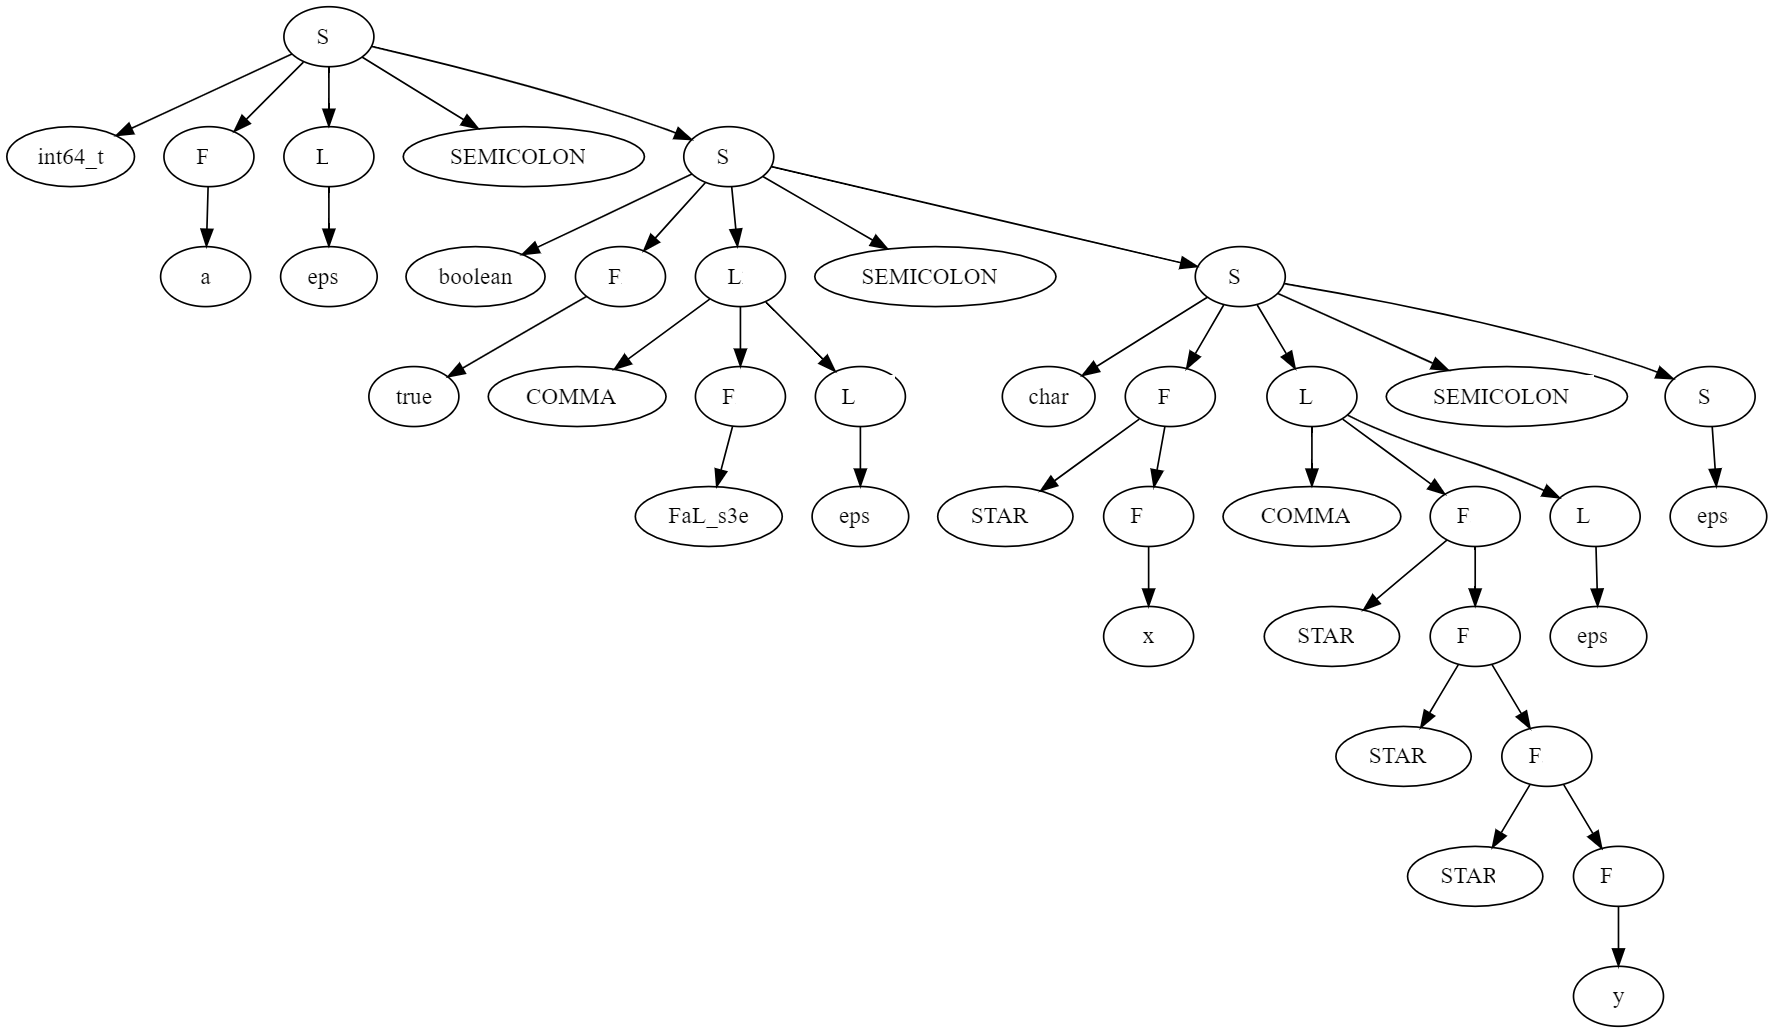
\includegraphics[height=16cm,width=18cm]{graphviz.png}
 \noindent 
  
  
  \section{5. Тестирование}
  
  \begin{center}
    \begin{tabular}{|l|l|}\hline
    Тест & Описание\\ \hline
       & Пустой тест, вернет ошибку\\ \hline
    int a;   & Простой тест, проверяет $S \rightarrow \varepsilon$, $Z \rightarrow \varepsilon$ и $N \rightarrow v$\\ \hline
    int a, b; & Тест на правило $Z \rightarrow N,Z$\\ \hline
    int64\_t a1, b2с; & Тест на распознавание названий переменных и типов\\ \hline
    int *a; & Тест на правило $N \rightarrow *N$\\ \hline
    int **a; & Тест на правило $T \rightarrow :n$\\ \hline
    int a; boolean b; & Тест  на правило $S \rightarrow nZN;S$\\ \hline
    int a*; & Ошибка - неожиданный символ \\ \hline
    64int 1var; & Ошибка\\ \hline
    int a & Ожидается ; \\ \hline
    a; & Ожидаются имена переменных \\ \hline
    int a int b; & Ошибка \\ \hline
    \end{tabular}
  
  \end{center}
\end{document}
